\documentclass[a4paper, 11pt, titlepage]{article}

\usepackage[english]{babel}
\usepackage[utf8]{inputenc}
\usepackage{amsmath}
\usepackage{amssymb}
\usepackage[linesnumbered]{algorithm2e}
\usepackage{graphicx}
\usepackage{times}
\usepackage{titling}
\usepackage{todonotes}
\usepackage{hyperref}
\usepackage{cleveref}
\usepackage{fancyhdr}
\usepackage{multirow}
\usepackage{array}
\usepackage[font=small,labelfont=small]{caption}
\usepackage{subcaption}

\makeatletter
\newcommand*{\centerfloat}{%
  \parindent \z@
  \leftskip \z@ \@plus 1fil \@minus \textwidth
  \rightskip\leftskip
  \parfillskip \z@skip}
\makeatother

\usepackage{listings}
\lstset{
    breaklines=true,
    basicstyle=\footnotesize,
    postbreak=\raisebox{0ex}[0ex][0ex]
 {\ensuremath{\hookrightarrow\space}},
    inputencoding=utf8,
    extendedchars=true
}
\lstset{literate=%
      {é}{{\'{e}}}1
      {è}{{\`{e}}}1
      {ê}{{\^{e}}}1
      {ë}{{\¨{e}}}1
      {û}{{\^{u}}}1
      {ù}{{\`{u}}}1
      {â}{{\^{a}}}1
      {à}{{\`{a}}}1
      {î}{{\^{i}}}1
      {ô}{{\^{o}}}1
      {ç}{{\c{c}}}1
      {Ç}{{\c{C}}}1
      {É}{{\'{E}}}1
      {Ê}{{\^{E}}}1
      {À}{{\`{A}}}1
      {Â}{{\^{A}}}1
      {œ}{{\oe}}2
      {Î}{{\^{I}}}1
      }

\pagestyle{fancy}
\renewcommand{\sectionmark}[1]{\markboth{#1}{}} % set the \leftmark

\fancyhf{}
\fancyhead[L]{\leftmark} % 1. sectionname
\fancyfoot[C]{\thepage}
\fancypagestyle{plain}{%
  \fancyhf{}%
  \renewcommand{\headrulewidth}{0pt}%
}


\newcommand\fnurl[2]{%
  \href{#1}{#2}\footnote{\url{#1}}%
}
\setlength{\headheight}{50pt}
\setlength{\marginparwidth}{2cm}

\title{A shallow NLP approach to characterization in \\French 19th century literature}


\author{Alexis \textsc{Semple} \\ 
Supervisors: Cyril \textsc{Bornet}, Frédéric \textsc{Kaplan} \\ 
Digital Humanities Lab \\
EPFL}

\begin{document}

\begin{titlepage}

\newcommand{\HRule}{\rule{\linewidth}{0.5mm}} % Defines a new command for the horizontal lines, change thickness here

\center % Center everything on the page
 
%----------------------------------------------------------------------------------------
%	HEADING SECTIONS
%----------------------------------------------------------------------------------------
\begin{figure}[t]
\centering
\includegraphics[scale=0.25]{fig/EPFL}
\end{figure} 
\vspace{3em}

\textsc{\large Department of Computer Science \\ semester project}\\[0.9cm] % Minor heading such as course title

%----------------------------------------------------------------------------------------
%	TITLE SECTION
%----------------------------------------------------------------------------------------

\HRule \\[0.4cm]
{ \Large \bfseries A shallow NLP approach to characterization in \\French 19th century literature}\\ [0.3cm] % Title of your document
\HRule \\[2.5cm]
 
%----------------------------------------------------------------------------------------
%	AUTHOR SECTION
%----------------------------------------------------------------------------------------

\begin{minipage}{0.4\textwidth}
\begin{flushleft} \large
\emph{Authors:}\\
Alexis \textsc{Semple}
\end{flushleft}
\end{minipage}
~
\begin{minipage}{0.4\textwidth}
\begin{flushright} \large
\emph{Supervisors:} \\
Cyril \textsc{Bornet}\\ 
Frédéric \textsc{Kaplan}
\end{flushright}
\end{minipage}\\[4cm]

% If you don't want a supervisor, uncomment the two lines below and remove the section above
%\Large \emph{Author:}\\
%John \textsc{Smith}\\[3cm] % Your name

%----------------------------------------------------------------------------------------
%	DATE SECTION
%----------------------------------------------------------------------------------------

{\large \today}\\[3cm] % Date, change the \today to a set date if you want to be precise

%----------------------------------------------------------------------------------------
%	LOGO SECTION
%----------------------------------------------------------------------------------------

%\includegraphics{Logo}\\[1cm] % Include a department/university logo - this will require the graphicx package
 
%----------------------------------------------------------------------------------------

\vfill % Fill the rest of the page with whitespace

\end{titlepage}

\newpage\null\thispagestyle{empty}\newpage 

% ABSTRACT HERE
\begin{abstract}
In the following, we present various approaches to the automatic description of characters in French 19th century novels. 
The aim of this work is to deepen our understanding of how characterization is constructed in literature, thus broadening the scope of most of the focus of current literature, which is closer to non-fiction or contemporary language. The approaches presented include lexical and structural/morphological methods.
By focusing on specific social and demographic aspects of their characterization within a novel, we discuss predictor methods for professional occupation, gender, associated sentiment of characters.
\end{abstract}

\tableofcontents
\newpage

\section{Introduction}

Recent advances in natural language processing techniques alongside the development of the field of Digital Humanities have lead to explorations of questions revolving around literary narrative. It is in this context that we investigate approaches to automatic extraction of metadata focusing on characters in French 19th century novels.

Natural language processing (NLP), as a discipline has found applications in ever wider domains. Since the expression and comprehension of thoughts and experiences in language is one of the foremost means of human communication, it is a capacity essential to understanding our wants and needs. As we develop the methods relevant to this discipline, we are able to further the complexity and depth of interaction between humans and machines. 

Digital Humanities as a field of endeavour is pushing boundaries by ``bringing the tools and techniques of digital media to bear on traditional humanistic questions'' \footnote{Kathleen Fitzpatrick \href{http://www.inthelibrarywiththeleadpipe.org/2015/on-scholarly-communication-and-the-digital-humanities-an-interview-with-kathleen-fitzpatrick/}{"On Scholarly Communication and the Digital Humanities: An Interview with Kathleen Fitzpatrick"}, In the Library with the Lead Pipe}. The field is striving to develop the complementarity to two rich and thriving aspects of human civilization. 

These humanistic questions, in our case, mean the study of literature. Our focus is specifically on the linguistic patterns of the elucidation of meta-information of characters in French 19th century literature, but many of the hypotheses, assumptions, and findings can be generalized to the wider field of fictional, and possibly non-fictional, character description. 

There have been many advances in the automatic study of fictional and non-fictional personas through natural language processing. This ranges from entity-centric \cite{chambers2013event} to event-centric \cite{cheung2013probabilistic} approaches. The persona is analyzed from varying standpoints, be it the role of the character within a particular fictional narrative \cite{valls2014toward}, or linking the observed character traits to non-fictional situations, like personality profiling \cite{flekova2015personality}, closely tied to that very practice in modern psychology.

All of the insights generated through these studies enrich our understanding of how narrative is developed, with regard to a character. The approach presented here focuses on yet another aspect of the fictional literary character, i.e. the social and behavioral elements tied to a characters existence, with the hope of broadening still this understanding. Some examples of these elements might be a character's professional occupation, place of origin, social status, age, gender. In short, elements that increase the knowledge of the character within its social existence, as we perceive it in the non-fictional sense. Throughout this work, we refer to these aspects as a character's \textit{metadata}.

Since our focus in this instance is specifically on French literature, it has some unavoidable implications on the procedure undertaken. Mainly, the predominant tools and procedures having been and being developed in all fields of NLP are focused on the English language. There are of course developments and resources in other languages, but it is as such not a space where the same resources are readily available (think coreference resolution, dependency parsing, etc.). It is worth noting that the relative sparsity of work done with regard to French (and other) language processing and the particularities of each individual language make such work interesting. 

As a result, the approaches tried in our case focus mainly on shallow NLP ideas. These tend to ``not attempt to achieve an exhaustive linguistic analysis'', and ``are designed for specific tasks ignoring many details in input and linguistic (grammar) framework'' \cite{schafer2007integrating}. There is also a distinct advantage in such an approach, in that they often allow for less time- and resource-consuming methods. 

This work is in no way exhaustive in the possibilities it presents, nor the opportunities explored. It does however aim to present how feasible a shallow approach to fiction is for understanding specific aspects of characters, by empirical measures of the efficiency of the methods explained below.

\section{Related work}
From the work done previously around the topic of automatic information extraction around literary characters, we identify some strands that we discuss here below. Among them are the following: the role a character plays within a narrative (e.g. protagonist, antagonist, mentor), understanding a character's profile, in the real world psychological sense, and extracting information about relations between characters. 

\subsection{Character roles}
In \cite{groza2015information}, a system is presented in which information is extracted about characters by interleaving NLP and reasoning on ontologies. By an efficient use of domain knowledge, they work with a set of rules that identify characters and match them with a concept, and then a character type in the ontology. The ontology was constructed specifically for their purposes, by formalizing knowledge on the folktale domain from different sources. 

Other approaches focus on developing systems less specific to genres or authors. In \cite{bamman2014bayesian}, a bayesian mixed effects model is presented that focuses on identifying latent character types in a very large english language corpus in an unsupervised manner. They define their character types as a distribution over various categories of typed dependency relations (agent, patient, possessive, predicative). A hierarchical Bayes approach is adopted, in which a word linked to a character is dependent not only on the character's latent persona, but also the background likelihood of both the word and the author.

There are tangential lines of work where character roles are learned with regard to specific events. This can of course lead to understanding the role of characters in a wider narrative. In \cite{chambers2013event}, the authors present a generative entity-driven model for event schema induction. Their modeling of the role uses the coreference chain of a character as the focus.


\subsection{Character profiling}
The work in this direction seems less frequent, presumably because it is focusing on the intersection of two domains, i.e. the study of literary characters on the one hand, and that of real world psychological personas on the other.

In \cite{flekova2015personality}, the authors describe a method for extracting the personality profile of fictional characters, based on the Five Factor Model of personality \cite{mccrae1992introduction}. They frame the problem of personality prediction as a classification task, and use both lexical resource-based features and vector-space semantics. The classification is thus based on features ranging from character actions to descriptive elements rather than personality assessing questionnaires, which is the real-world standard.

\subsection{Character relations}
Much of the work done in identifying typed or untyped relations between fictional characters relies on the construction of social networks from literary works. In \cite{elson2010extracting}, the authors present a system that relies on extracting interactions by identifying dialogues between characters. 

In \cite{kokkinakis2011character}, on top of the social network extraction, using character interactions and also various vocabulary and lexical semantic resources, the authors posit that such a network structure can potentially inform about character metadata, such as birthplace, workplace, by constructing a network of character-location interaction, and using lexical semantic resources. This can be considered a potential extension of the work presented in this paper.



\section{Resources}
Here we present the main external resources that were used to perform this work. The code for this project can be found in the \href{https://github.com/semplea/characters-meta}{GitHub repository} \footnote{\href{https://github.com/semplea/characters-meta}{https://github.com/semplea/characters-meta}}.

\subsection{Data} \label{ssec:data}
The books we worked with were all processed in the form of a simple text file, provided by Project Gutenberg. Each file was then processed so that each chapter was written onto a single line.

We worked extensively with previous work done by Cyril Bornet around character and location recognition, focused on the same works of literature \footnote{A set of novel analysis tools \href{https://github.com/dhlab-epfl/3n-tools}{on GitHub: https://github.com/dhlab-epfl/3n-tools}}. So on top of the raw books, we were able to assume and work with a good set of the characters within a novel, provided in a deterministic list.

In order to measure the efficiency of our model, we also annotated by a small number of books with information about gender and professional activity. Since we would be focusing on very limited data, it was important to pick a selection of books representative of the question we wanted to answer, but also allowing that question a certain scope to explore possibilities. We decided to pick books based on the following criteria:
\begin{itemize}
\item book contains varied character types and relations 
\item there are explicit metadata about a majority of the characters
\item the full selection will be composed of different authorial styles 
\end{itemize}

The books we ended up annotating and working more closely with for the evaluation of our work are \textit{Au Bonheur des Dames} (ABDD) and \textit{L'Assommoir} (LASS), by Émile Zola, \textit{Madame Bovary} (MBOV), by Gustave Flaubert, \textit{Le Tour du Monde en quatre-ving jours} (LTDM), by Jules Verne, and \textit{Candide} (CAND), by Voltaire. More information is given in \cref{tab:books}. 

\begin{table}
\centering
\begin{tabular}{|l||*{4}{c|} }
\hline
Book & Tokens & Characters & Job labels & Gender labels \\ \hline \hline
LTDM & 75674 & 25 & 23 (34) & 23 \\ \hline
ABDD & 174635 & 58 & 41 (59) & 57 \\ \hline
LASS & 173154 & 45 & 23 (31) & 43 \\ \hline
MBOV & 131883 & 46 & 27 (39) & 46 \\ \hline
CAND & 36015 & 11 & 8 (11) & 13 \\ \hline \hline
\bf Total & 591361 & 185 & 122 (174) & 182 \\ \hline
\end{tabular}
\caption{Information given per annotated book (abbreviated titles). In order of the columns, we have the total number of tokens in the book, the number known characters, number of job-labeled characters (total number of jobs identified as valid), number of gender-labeled characters.}
\label{tab:books}
\end{table}

\subsection{Tools}
The main technical tools we worked with are NLP tools, that were employed for basic purposes. For some of the predictors, required PoS tags for the text. We were able to use the \href{http://www.cis.uni-muenchen.de/~schmid/tools/TreeTagger/}{TreeTagger} \cite{schmid2013probabilistic}, which is built to find the tags for many different languages, including French. 

In order to get word representations for computing word similarities, as discussed below in section \cref{sssec:profession}, we used pre-computed word embedding model\footnote{trained by Jean-Philippe Fauconnier. Details on his \href{http://fauconnier.github.io/}{website}}, trained on the frWaC corpus, a 1.6 billion linguistically processed french language corpus constructed from \textbf{.fr} web domains \cite{baroni2009wacky}. The word embeddings were learned using the word2vec algorithm developed by Mikolov et al. \cite{mikolov2013distributed}. In our project, we used these embeddings with \href{https://radimrehurek.com/gensim/models/word2vec.html}{\texttt{gensim}'s \texttt{word2vec}} module for \texttt{python}.


\section{Extracting character metadata} \label{sec:metadata}
Our metadata predicting model builds on two hypotheses about where in a work of fiction a character's metadata (job, gender, family, etc.) can be explicitly found. In literary terms, this metadata can be considered part of a \textit{characterization}. 

For a given character $c_i$, we posit the following (notation explained below):
\begin{enumerate}
\item explicit elements of $c_i$'s metadata are likely to be within a window $w$ surrounding an occurrence of $c_i$
\item explicit characterization is more likely to occur within the first $k$ occurrences of $c_i$
\item explicit characterization is more likely in a sentence where $c_i$, but no $c_j \in \mathcal{C}$ occurs, $i \neq j$.
\end{enumerate}

In section 5 we discuss how our predictors support these hypotheses.

For a given book, we define a character $c_i$, such that $c_i \in \mathcal{C}$, where $\mathcal{C}$ is a set of size $N$. Each book is split into sentences $s_j \in \mathcal{S}$, $\mathcal{S}$ of size $M$ (number of sentences in book). 

The term \textit{window} in hypothesis 1. describes a batch of either words or sentences, taken before and after a character occurrence. So for a given window wing size $w$, and the $k$th occurrence over the whole book of $c_i \in \mathcal{C}$  in sentence $s_j$, we have a window $W_{\mu^i_k}$, s.t. 

\begin{equation}
W_{\mu^i_k} = [s_{j-w}, s_{j-w+1}, ...,  s_{j-1}, s_{j}, s_{j+1}, ..., s_{j+w-1}, s_{j+w}]
\end{equation}

where $\mu^i_k$ is the $k$th occurrence of $c_i$, and $0 \leq k \leq L_i$, so $c_i$ has a total of $L_i$ occurrences in the book. In this way, a window is of size $2w + 1$. Note that the inferior and superior bounds for a window are $s_0$ and $s_m$, so the leftmost sentence in any case is actually $s_{\min(0, j-w)}$, and the rightmost $s_{\max(m, j+w)}$. An example is given for character \textit{Phileas Fogg} in \cref{fig:window}

\begin{figure}
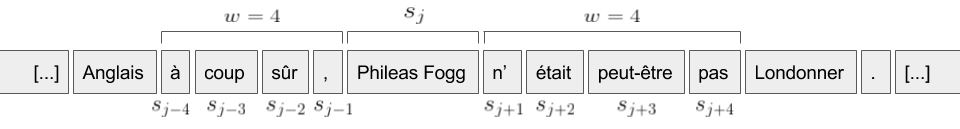
\includegraphics[width=\textwidth]{fig/window.png}
\caption{Window example, with w=4. Note, in  this sentence all tokens are taken for consideration, whereas in practice we worked with sentences without stopwords, and more in some cases (e.g. only specific PoS tags). We also use words to determine the window. In practice, this could also be whole sentences instead.}
\label{fig:window}
\end{figure}

For character $c_i$, let its document $D^{c_i}$ be the collection of all the windows with an occurrence of $c_i$ at their center. This whole description can be taken analogously for windows of words instead of sentences. We experimented with different window parameters for the various predictors described below. 

\vspace*{1em}
% Hypothesis 2
Hypothesis 2 implies that metadata is more likely to be found in the initial $\mu^i_k$. This is verified in the predictors by comparing different methods. We decided on two representations of this. A natural first possibility is to constrain $D^{c_i}$ to the first $k$ occurrences of $c_i$. We write this $D^{c_i}_{[0:k]}$. 

Additionally, we used weights $\omega^i_k$ for a mention $k$ of $c_i$ that decrease as $k$ increases. For this purpose, an exponentially decreasing function was chosen, such that if we want to compute the weight $\omega$ for a measure for a given predictor of $c_i$ at mention $k$, we have
\begin{equation}
\omega^i_k = -\log (\frac{k+1}{L_i})
\end{equation}


% Hypothesis 3
Hypothesis 3 stipulates that if $c_i$ occurs without the mention of any other characters in the book, then explicit characterization is more likely, or at least, some shallow techniques might be more precise. We test this by using a filtered document 
\begin{equation}
D^{c_i}_{filt} = D^{c_i} \backslash \bigcup_j D^{c_j}
\end{equation}
where $i \neq j$. 

Of course the hypotheses discussed are not conflicting in nature and can be applied alongside each other, and were tested as such for our predictors. With this setup, we went on to try different approaches to extracting metadata for individual or a whole collection of characters in a book.

\subsection{Extraction by LDA}
As a preliminary exploration of the characterization of an entity in a book, we applied a latent dirichlet allocation (LDA) \cite{blei2003latent} on the document of the entity. By this generative probabilistic model, we get a requested amount of topics, each topic being a distribution over the words of the document. The implementation discussed below can be found in the \texttt{LDACapture.py} file.

Since this is basically an unsupervised way of extracting data, we get results that are not specifically pertinent to characterization, but more a broad indicator of the whole narrative (local to the given character). However, some of the topics were found to be pertinent. This is mainly in cases where the metadata considered plays a recurrent and central part in the narrative.

To extract them, we first focused on a particular aspect we wanted to observe. For instance, the model is more likely to capture information about a profession if it is provided only with common and proper nouns, since this filters out 'noise' irrelevant to this question (adverbs, adjectives, etc... verbs could be indicative, but there are many more generic ones that have a higher probability within any standard text). This filtering is achieved with the probabilistic tagging provided by TreeTagger. Additionally, we work exclusively with lemmas (also, provided by TreeTagger), when they are known, in order to minimize morphological variations.

If we take an example from \textit{Au Bonheur des Dames}, and look at the topics generated for the main character Denise, a saleswoman in a clothing store, by providing the LDA model with sentences containing only occurrences of the token `Denise', it's obvious that the concept of shops is indicated (words like \textit{magasin}, \textit{boutique}, \textit{vêtement}, \textit{rayon}.

\begin{lstlisting}
Topic 0 - 0.083*"magasin" + 0.055*"dames" + 0.055*"bonheur" + 0.055*"émotion" + 0.042*"question" + 0.042*"larme" + 0.028*"air" + 0.028*"heure" + 0.028*"idée" + 0.028*"vérité"

Topic 1 - 0.054*"boutique" + 0.054*"place" + 0.054*"bouche" + 0.054*"oncle" + 0.054*"tour" + 0.037*"cœur" + 0.037*"moi|mois" + 0.037*"œil" + 0.037*"peur" + 0.037*"silence"

Topic 2 - 0.066*"peur" + 0.050*"elle-" + 0.050*"fraîcheur" + 0.034*"œil" + 0.034*"larme" + 0.034*"enfant" + 0.034*"famille" + 0.034*"vêtement" + 0.034*"geste" + 0.034*"désir"

Topic 3 - 0.091*"main" + 0.047*"oncle" + 0.047*"frère" + 0.047*"rayon" + 0.047*"chambre" + 0.047*"reste" + 0.047*"idée" + 0.024*"rue" + 0.024*"milieu" + 0.024*"dailleurs"
\end{lstlisting}

However, since this is a central theme of the whole book, it can't be seen as conclusive in any way. If we look instead at an example from \textit{Le tour du monde en quatre-vingt jours}, and take Passepartout, the valet, as the character, we get the following

\begin{lstlisting}
Topic 0 - 0.093*"pensée" + 0.071*"sac" + 0.071*"bank-notes" + 0.048*"jour" + 0.048*"maison" + 0.048*"brique" + 0.048*"esprit" + 0.048*"monsieur" + 0.025*"main" + 0.025*"train"

Topic 1 - 0.084*"train" + 0.067*"milieu" + 0.051*"maître" + 0.051*"livre" + 0.034*"jour" + 0.034*"pied" + 0.034*"chambre" + 0.034*"peine" + 0.034*"journée" + 0.034*"coup"

Topic 2 - 0.080*"heure" + 0.080*"rue" + 0.064*"maître" + 0.049*"ville" + 0.049*"exercice" + 0.049*"agent" + 0.033*"bord" + 0.033*"main" + 0.033*"montre" + 0.033*"yokohama"

Topic 3 - 0.248*"maître" + 0.059*"air" + 0.040*"paquebot" + 0.040*"hong-kong" + 0.040*"départ" + 0.040*"bord" + 0.040*"bonheur" + 0.021*"heure" + 0.021*"rangoon" + 0.021*"jusqu"
\end{lstlisting}

where the theme of travel is obviously dominant. Only weak indications of his profession can be found, in the word `ma\^itre' (master), recurring in several topics. 

After these disappointing results, we try the approach of writing specific predictors for metadata categories.

\subsection{Metadata-specific predictors}
We implemented three different predictors that focus on specific aspects of a character's metadata, i.e. profession, gender and sentiment. In this way we look at aspects from a character's \textit{activity}, \textit{person} and \textit{psychological affect}. In the implementations of these predictors, three different main methods are used that cover a good spread of conceivable additional predictors, i.e. ad-hoc lexicon-based and linguistic-rule-based, or using external tools.

The implementations discussed below can be found in the \texttt{computeMeta.py} file.

\subsubsection{Profession} \label{sssec:profession}
For predicting the profession of a character $c_i$, we utilized an external corpus \footnote{A list of approximately 2600 masculine and feminine profession titles at \href{http://www.vd.ch/guide-typo3/le-texte/rediger-pour-le-web/redaction-egalitaire/2000-noms-au-masculin-et-au-feminin}{http://www.vd.ch/guide-typo3/le-texte/rediger-pour-le-web/redaction-egalitaire/2000-noms-au-masculin-et-au-feminin}} of known professions in French. Let $p_k \in \mathcal{P}$ be the $k$th  profession in the list. 

Our approach is then split along two different measures. On the one hand, we look at the co-occurence \textbf{count}, i.e. 
\begin{equation}
count_{c_i, p_k} = \sum_j \mathbb{I}^{c_i}_j \mathbb{I}^{p_k}_j
\end{equation}
where the indicator functions $\mathbb{I}_j = 1$ if $c_i$ (resp. $p_k$) occurs in sentence (or window) $j$. This is computed $\forall c_i \in \mathcal{C}, \forall p_k \in \mathcal{P}$, and kept in a dictionary of $c_j \rightarrow [p_0, p_1, ...]$. The job with the highest count score is taken as the winner. 

On the other hand, we look at the mean \textbf{proximity} measure, so for given $c_i$ and $p_k$, get the mean distance between the two within a window. See \cref{alg:proximity} for a sketch of the implementation. 

\begin{algorithm} 
  \KwData{$charWindows, jobList, jobCount, char$}
  \KwResult{$score$}
  $score \leftarrow$ a map with jobs for keys and values $\leftarrow 0$\;
  \For{$win \in charWindows$}{
    \For{$job \in jobList$}{
      \If{$job \in win$}
      {$\texttt{increment}(jobCount[char], 1)$\;
      $dist = \texttt{abs}(\texttt{indexOf}(win, char), \texttt{indexOf}(win, job))$\;
      $\texttt{increment}(score[job], dist)$\;}                
    }
  }
  \For{$(job, value) \in score$}{
      $score[job] \leftarrow value / jobCount[job]$ 
  }
  \caption{Computing job proximity scores for a given character.}
  \label{alg:proximity}
\end{algorithm}

As before, this is computed $\forall c_i \in \mathcal{C}, \forall p_k \in \mathcal{P}$ and stored in a dictionary. The job with the lowest mean proximity score is taken as the winner.

Note, this gives an idea of the implementation for the count score as well, and can be applied to other aspects of a $c_i$'s metadata (e.g. family ties, nationality). The process needs a collection of keywords to extract from a given $D^{c_i}$, in the case of \cref{alg:proximity}, the \textit{jobList}, and a scheme for aggregating the occurrences into a score for each keyword, which is done here by the \textit{distance} function.

We additionally implemented an \textbf{aggregate predictor}, combining both proximity and count measures, where we add their weighted normalized scores together. The weights were chosen to approximate best results.


\subsubsection{Gender} \label{sssec:gender}
In order to predict the gender of a character, we tried to capture different lexical, linguistic and morphological aspects of a window surrounding that character. In turn, we captured the number of masculine and feminine pronouns in the window, the number of adjectives with feminine or masculine form, the number of obvious titles linked to the character. These scores were then combined to provide the best possible prediction.

\paragraph{Pronoun} We captured the masculine and feminine pronouns (`il', `elle') in the window containing $c_i$ (and for the words with the relevant PoS tag: \texttt{PRO:PER}), and aggregated the captures by adding $+1$ for each feminine, and $-1$ for each masculine occurrence. Note that this can be considered problematic due to the use of the masculine pronoun for the impersonal case as well (in english `it'), e.g. \textit{`il est clair que...'}. In practice, even with this strong assumption, the results weren't too biased towards predicting male characters.

\paragraph{Adjective} Lists of typical masculine and feminine adjective endings were compiled (e.g. \texttt{[`el', `er', `en', `on', ...]}, and \texttt{[`elle', `enne', `onne', `euse', ...]} respectively. For words with the relevant PoS tag (\texttt{ADJ}), we again aggregated these captures by a similar method as above.

\paragraph{Immediate surroundings} A lot of pertinent and almost obvious information can be found for certain words immediately preceding the character occurrence. 

Given the formal nature style of many of the texts we deal with in this work, there are plenty of \textbf{titles} used to address the characters. On top of this, the set of characters for a book was provided with compounded names, i.e. `MrFogg', `MrsAouda'. This allowed us, with compiled lists of feminine and masculine titles (\texttt{[`madame', `mademoiselle', `mme', ...]}), to look for both a title in the compounded name, and in the word directly preceding the occurrence of the character.

Additionnally, we keep score of any feminine or masculine pronouns or articles directly preceding the character occurrence, i.e. `le' or `la', `ce' or `cette', `mon' or `ma'. This aims to capture affectionate and informal ways of address (e.g. `ma Denise').

\paragraph{Character name}
We used a gender determination service \footnote{\href{https://genderize.io/}{https://genderize.io/}. It is built utilizing data from social network profiles across the globe. For a given name, a request returns a gender (if name is known), with a certainty factor.} on the (first) names of characters. For certainty factors above a certain threshold (i.e. $> 0.95$) we used a greedy scheme that would attribute the gender label directly to the result of the character, since this proved to work at a very low error rate. For anything below the threshold, we used a weighted contribution to the overall score.
\vspace*{1em}

In order to best combine the scores of these methods, we wanted to approximate good weights for each. We did this by a logistic regression on our labeled data set, using the different scores computed as features, and used these approximate weights for the model. Seeing as we have very few data points labeled, this is by no means a sufficient method, but it gives us an idea of the importance of each `feature'.

\subsubsection{Sentiment} 
In order to predict the sentiment associated with a character $c_i$, we used an external API, powered by NLTK \cite{perkins2010textclass}. This is a Naive Bayes classifier, trained on movie reviews and tweets. The language of the training data is thus quite different from what we can expect from 19th century literature, but not so much so that it is irrelevant.

Given the limitations of the API, we weren't able to query the sentiment of the full document $D^{c_i}$. We assumed a subset (usually 10\%) of the document would be enough to gather insights. In order to make the query more revealing however, we used only words with sentiment-relevant PoS tags in the document, i.e. \texttt{'NOM', 'ADJ', 'PUN', 'VER', 'ADV'}. Additionally, we work with the lemmatized versions of the document, in order to avoid morphological variations.

We query the API for each window $W \in D^{c_i}$. The result of a call is a `label', either `pos', `neg' or `neutral', and the corresponding probabilities. A natural way to decide the general sentiment associated with $c_i$ is then to pick the majority label for $D^{c_i}$.

\section{Results}
In the following, we present an evaluation of the predictors discussed in section \cref{sec:metadata}. 

\begin{table}
\centering
\begin{tabular}{| l | *{5}{c|}}
																				\cline{1-2}
valet		& 1																\\	\cline{1-3}
serviteur	& 0.367	& 1 													\\	\cline{1-4}
domestique	& 0.116	& 0.072 	& 1											\\	\cline{1-5}
p\^atissier	& 0.148	& 0.087		& 0.087			& 1							\\ 	\cline{1-6}
cuisinier 	& 0.211	& 0.156 	& 0.078			& 0.567			& 1			\\	\hline
 			& valet &serviteur	& domestique	&p\^atissier	& cuisiner	\\	\hline
\end{tabular}
\caption{Cosine distance for given word vectors using pre-trained word2vec model, with skip-gram architecture and dim=700.}
\label{tab:word_sim}
\end{table}

\subsection{Profession predictor}
In order to evaluate the precision of this predictor, we decided on utilizing the numerical representations of word embeddings to get a measure out of it, since the multiple possible outcomes made it impossible to qualify it as a classification. We wanted to be able to take semantic similarity into account. Word embeddings can provide this, to a certain extent. 

The pre-computed model we use is trained using the skip-gram model, which performs better than a continuous bag-of-words model for semantic similarities \cite{mikolov2013efficient}. The vectors are 700-dimensional and were computed on 1.6 billion words from French web domains

In effect this means we're able to get a numeric similarity between two words (or job-titles) by getting the cosine distance between their vector representations. We compare an extracted title with our hand-labeled title, and thus get a similarity score. This measure should be taken with a pinch of salt however, since the similarities weren't extensively tested on our job corpus. In \cref{tab:word_sim}, we see that the two highest scores are for the pairs `valet'-`serviteur' and `cuisinier'-`p\^atissier', which is as one would expect. However `domestique' has a surprisingly low similarity with both `valet' and `serviteur', which are semantically similar. Since the model uses PoS tags (i.e. `domestique\_n' to indicate it's a noun) to avoid ambiguity, this isn't due to confusion with its adjective form.

\begin{figure}
\centering
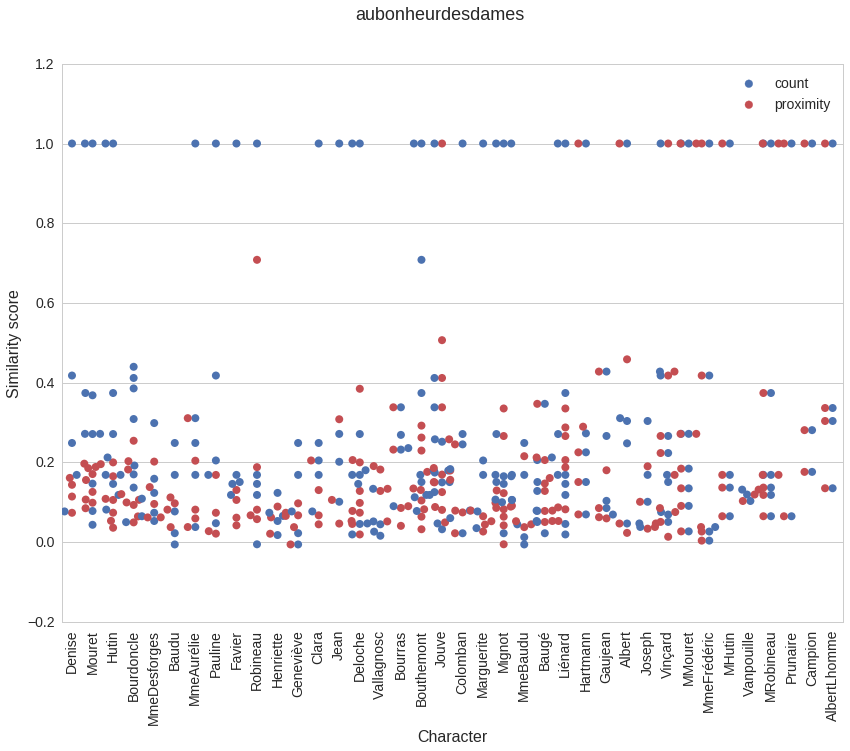
\includegraphics[width=.8\textwidth]{fig/count_vs_prox_bonheur.png}
\caption{Count vs Proximity predictor scores on \textit{Au Bonheur des Dames} characters. Points with score 1 are an exact match between two words. Characters are ordered by decreasing occurrence count. \textit{Note}: plots for other books are generally similar.}
\label{fig:count_vs_prox}
\end{figure}

The job predictor returns the 5 top guesses for a $c_i$'s job. In \cref{fig:count_vs_prox}, we show the result of the `count' and `proximity' predictors. In some cases, the job labels for the characters contain more than one possibility, which is why some characters have more points in the graph than others. The figure shows that the `count' predictor is far more present in the exact matches with the label, and `proximity' points are more pertinent when used for more minor characters. 

\begin{table}
\centering
\begin{tabular}{| l | *{5}{c|}}
\hline
& \multicolumn{5}{ |c| }{Rank} \\ \cline{2-6}
					& 0		& 1 	&2 		& 3		& 4		\\ \hline 
Individual ratio	& \textbf{0.41}	& 0.22	& 0.1	& 0.09	& 0.05	\\ \hline
Cumulative ratio	& 0.41	& 0.55	& 0.61	& 0.68	& 0.71	\\ \hline

\end{tabular}
\caption{Perfect match ratio for different ranks. The full character-set has 108 characters. The individual ratio is the ratio for only the given rank, and the cumulative is the ratio up until and including the given rank.}
\label{tab:match_ratio}
\end{table}

The results in \cref{fig:count_vs_prox} are encouraging, seeing as a majority of the characters (in this book, but also others) have an exact match between one its job-labels and at least one among the top 5 predictions. As an additional step, we look at the percentage of characters with exact matches in each of the 5 ranks in \cref{tab:match_ratio}. These were achieved using the `aggregate' predictor on the full book, with constant increments (c.f. figures below).

\begin{figure}
\centering
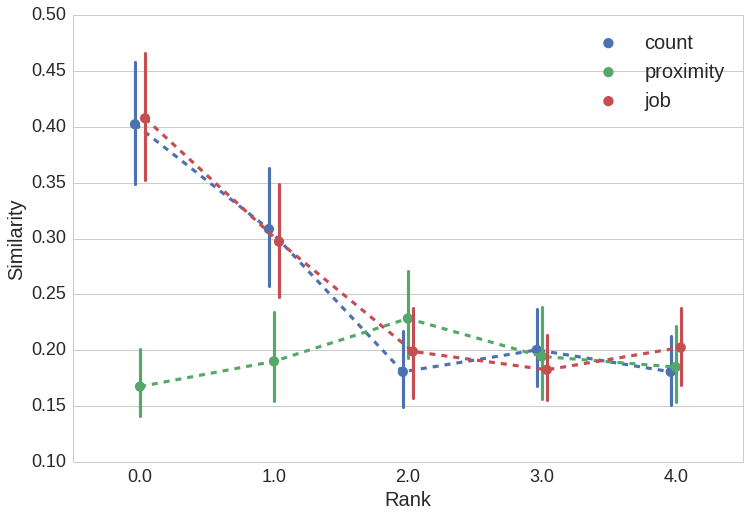
\includegraphics[width=.6\textwidth]{fig/rank_cpa.png}
\caption{Mean of all book and character scores grouped by 'rank' of prediction. Here the plots are of the `count', `proximity' and `aggregate' (first two combined) predictors. The bars represent the confidence interval for the point estimate.}
\label{fig:rank_cpa}
\end{figure}

To get an understanding of how the different guesses perform, in order, we plot the mean of all similarity scores (all books, all characters) grouped by the rank they were predicted in, in \cref{fig:rank_cpa}. The `aggregate' predictor is a combination of the other two, but with a higher weight given to the `count' predictor. We can see that it scores slightly higher than the `count' predictor for its first predictions.

\begin{figure}
\centering
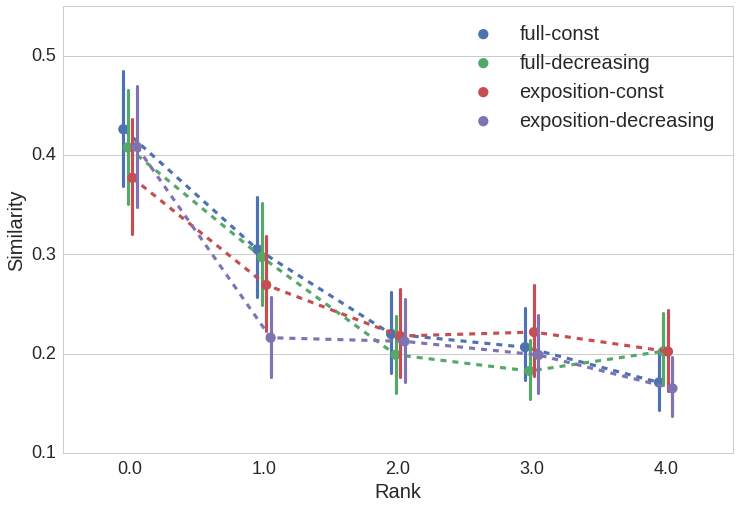
\includegraphics[width=.6\textwidth]{fig/job_params.png}
\caption{A comparison of the different parameters for the job predictor. `full' indicates the prediction was made based on observations from the whole book, whereas `exposition' focuses only on the $k$ first occurrences (here $\max(\frac{1}{10}L_i, 10)$, where $L_i$ is the length of $c_i$'s document). `decreasing' indicates that the weight of the contributions of each occurrence decreases (by rate seen in \cref{sec:metadata}) with occurrences later in $c_i$'s document.}
\label{fig:job_params}
\end{figure}

The effect of the different parameters of the job predictor are shown in \cref{fig:job_params}. We can see that the best similarity score on rank 0 and 1 is achieved with the `full-constant' parameter, but for ranks 2, 3 and 4 it's the `exposition-constant' that is on top. It seems working with the full range of data available in a characters document is generally preferable.

Both \cref{fig:rank_cpa} and \cref{fig:job_params} were created with approx 3000 data points, split evenly between the 5 `rank' categories. There are 108 distinct characters among them, taken from the 5 different books described in \cref{ssec:data}. Given the limited nature of this data, we should take the results presented above as indicators, but not entirely deterministic. The precision of these evaluations would benefit from more labeled books, and a system of expert reviewers for the labels.

The results above seem to work in favour of hypotheses 1 and 2 discussed in \cref{sec:metadata}. On the one hand, the result is slightly better when using a proximity score, and we also work with a constrained window size (maximum 5 sentences, with character occurrence at center), which performs better than larger sizes. This indicates there is an information gain from looking at and weighting the data close to the character higher, as hypothesis 1 stipulates. 

On the other, the predictor using only `exposition' occurrences (initial $\frac{1}{10}$th of total) has a performance very close to that of the `full' occurrences. Given that these occurrences are much fewer in number, and thus provide much less data overall, one can see that a lot of the metadata we're looking for will presumably be found within an exposition phase, as hypothesis 2 stipulates (first $k$ occurrences is called the `exposition' here).

\subsection{Gender predictor}
The evaluation of the gender predictor is more straightforward, since it is taken as a 2-class classification, i.e. we want to predict when a character is female. All characters were labeled with either a `m' (for male), `f' (for female) or `-' (for unknown) tag. The latter was given in cases where there wasn't a clear answer, for example when the predicted character name was used interchangeably for different family members (mother, father, children), or for animals of unknown gender. These characters were ignored in the classification metrics given below.

We provide the results for different feature generation schemes that we used, i.e. either all character $c_i$'s occurrences are taken, or only the ones where $c_i$ appears alone (filtered document). The accuracy, precision, recall and f-score metrics are shown in \cref{tab:gender_metrics}. Overall, the best performance is achieved when using the weighted features from the whole character documents. This is by a small margin however, so can't be considered conclusive. In part this is due to the greedy labeling of the name-gender predictor, since without it, there is a bigger gap in the ratio of guessed data points (approx. $7\%$) between the `solo' and `full' data. 

This failing of the `solo' data seems to be an argument against our 3rd hypothesis in \cref{sec:metadata}, but can also be attributed to the fewness of data in our character documents, and the general nature of the extracted features (i.e. only small percentage of sentences will get positive or negative score off these features).

\begin{table}
\centering
\begin{tabular}{| >{\bf}l || *{5}{c|}}
\hline
		& Accuracy & Precision	& Recall & F-score & Known ratio\\ \hline \hline
GFNW	& 0.873 & 0.758 & 0.979	& 0.854	& 0.83 	\\ \hline
GSNW	& 0.878	& 0.793	& 0.938	& 0.859	& 0.81	\\ \hline
GFW		& 0.88	& 0.767	& 0.978	& 0.859	& 0.83 \\ \hline
GSW		& 0.869	& 0.779 & 0.938 & 0.851	& 0.81 \\ \hline

\end{tabular}
\caption{Comparison of different features and weights used on the gender prediction task.`G' is for gender, `F' means we used the full data, as opposed to `S' (for solo), where we worked only with sentences where the character occurs alone. `NW' means the scores are non-weighted, and `W' means they are weighted, with weights approximated from a logistic regression. The column 'Known ratio' indicates the ratio of data points for which the predictor was able to make a guess.}
\label{tab:gender_metrics}
\end{table}

We show the distribution of predicted and true labels in \cref{fig:gender}.
Interestingly, we see in \cref{fig:gender_dist} that the predictor tends to output more `female' labels than there are true data points of that category, and the opposite for the `male' category. We remarked on the problematic case of the neutral `il' in \cref{sssec:gender}. These results show that the bias even tends towards the opposite direction. This can be attributed to the efficiency of the multi-feature predictor, in that each feature contributes only a fraction of the result score. Additionally, the pronoun feature was shown to be less efficient and thus given a smaller weight than the other features. 

\begin{figure}
\centering
\begin{subfigure}[b]{0.45\textwidth}
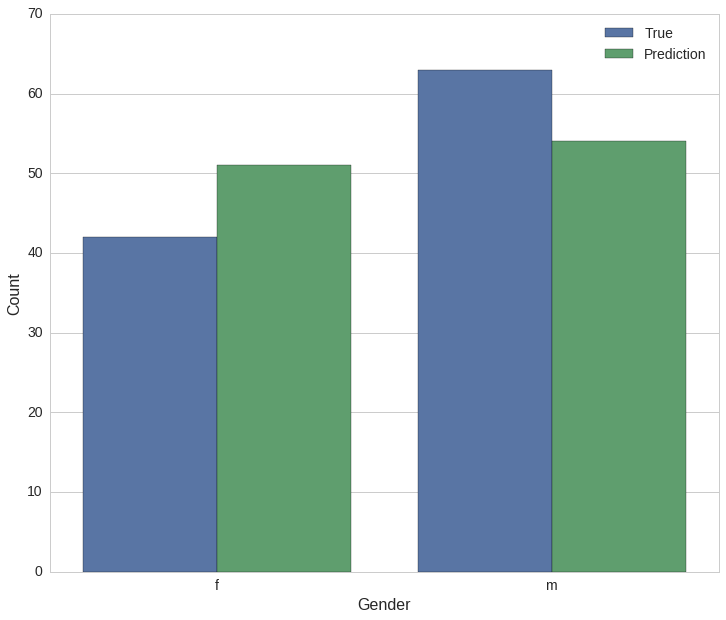
\includegraphics[width=\linewidth]{fig/gender_dist.png}
\caption{Distribution of gender predictions and true labels.}
\label{fig:gender_dist}
\end{subfigure}
\hspace{1em}
\begin{subfigure}[b]{0.45\textwidth}
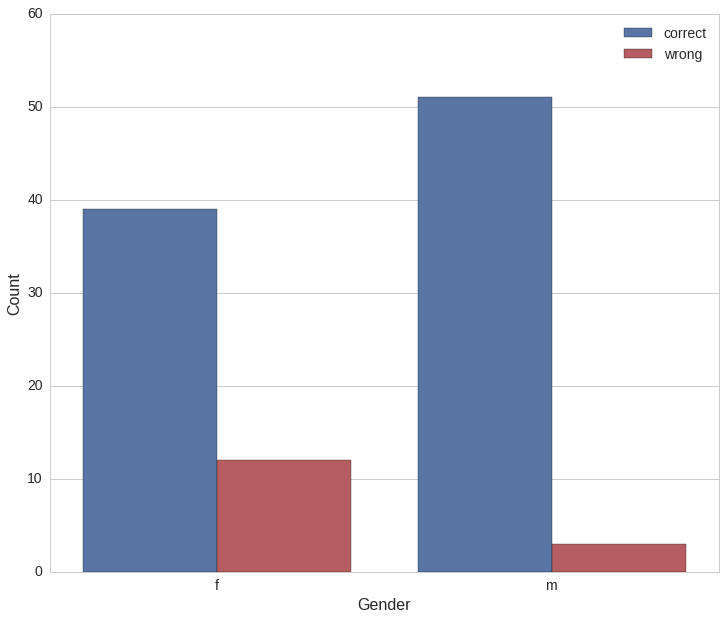
\includegraphics[width=\linewidth]{fig/gender_error.png}
\caption{TP, TN, FP and FN rates for the gender predictions (`f' is said to be positive).}
\label{fig:gender_error}
\end{subfigure}
\caption{Gender predictor metrics.}
\label{fig:gender}
\end{figure}
  


What we're doing here can be considered a no-go, by ML standards. However, since we're using only these `hand-generated' features, and they are designed to adhere to as general standards as possible, the chance of overfitting is minimal. On top of this, we're using the weights generated by the model merely to confirm suspicions that we already had about each feature's importance. 

For example, the score measuring specific pronouns in the window with $c_i$ is error-prone by design. The pronouns `il' and `elle' are among the most frequent words in the French language. The scores of specific titles or articles immediately preceding a $c_i$ occurrence is far more precise, and thus also less prone to error (or noise). It's safe to assume that these last two will have a higher weight than the first. This was confirmed by the weights given by our models. 

As a sanity-check, we generated predictions on some unused books during training of the weights, and verified that results are similar to the ones we obtained in \cref{tab:gender_metrics} . Usually, they were a few percent lower, i.e. for \textit{Nana}, by Zola (66 characters), we get an accuracy of $82.1\%$, precision, recall and f-score of $75.8\%, 88\%, 81.5\%$ respectively and a known ratio of $0.848$.

By the nature of our features (specific word types or words occurring in window with $c_i$), about $20\%$ of data points remain undecided (neutral). A quick look at these characters indicates that none of these play a major role within the book, so we can assume this is due to a lack of data.

\begin{figure}
\centering
  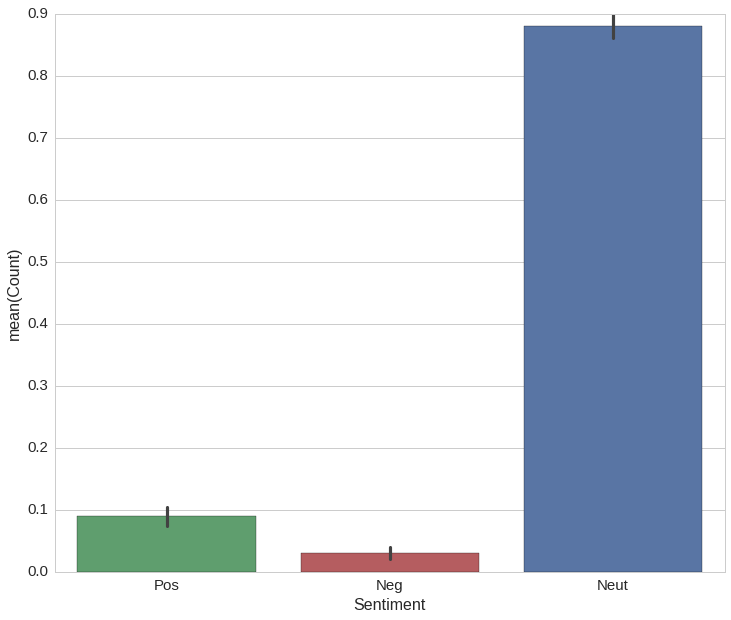
\includegraphics[width=0.6\textwidth]{fig/sent_prop.png}
  \caption{Mean proportions of positive, negative and neutral sentences for reduced character documents. Here the mean for all characters are shown.}
  \label{fig:sent_prop}
\end{figure}

\subsection{Sentiment predictor}
The results of the sentiment predictor on the characters is meaningful mainly for major characters. The API used returns the result `neutral' for most sentences it receives (c.f. \cref{fig:sent_prop}. So for a small number of sentences, we will have only a handful that indicate any sentiment, according to the NLTK tool we use. This may be due to a justifiably conservative predicting scheme on the part of the text classifier, however it has as a consequence that we're unable to extract a truthful understanding around the sentiment pertaining to a character in a novel, which is often associated with hundreds of sentences, and a wide range of polar descriptions.

Some characters with obvious polarities associated with them (i.e. Mrs Aouada, from \textit{Le Tour du Monde en 80 Jours} should be positive, Hutin from \textit{Au Bonheur des Dames} should be negative) are predicted with the wrong or no polarity (c.f. \cref{tab:full_vs_red}).

As mentioned in \cref{sssec:sentiment}, we compared the extracted NLTK sentiment metrics with the LIWC \cite{liwc2015} `emopos' and `emoneg' variables, gotten on the full character documents for the top 5 characters in each of our 5 books. The results were proportionally similar (almost identical) when computed on the same filtered sentences we used for the NLTK sentiment score and the raw sentence, which is an indicator of the efficiency of the filtering. In this way, we were able to provide less words, i.e. a less computationally intense operation, while achieving as effective results.

We expected similar results, since both methods are dictionary based. However there seems to be less variability in the LIWC results, as shown for the characters in \cref{tab:full_vs_red}. All characters tested have higher positive emotion variable values than the negative, but there are some telling differences in the ratio between them. For example `MrsAouda' has a significantly higher pos-to-neg ratio than `Bourdoncle'. This is also reflected in the NLTK values extracted.

With additional resources, less limited access to the NLTK text sentiment classification API, we could have compromised less. In order to truly evaluate such a result, as we did for the `gender' predictor, we would need access to expert-reviewed labels for a set of books. Associated sentiment is too ambiguous a notion for us to make a decision about the less than obvious characters. We also didn't intend for this predictor to answer a precise question about a character's sentiment throughout a narrative, but rather to understand sentiment associated with a character like a bubble surrounding his or her actions. 


\begin{table}
\centerfloat
\begin{tabular}{| l | l || *{6}{c|}}
\hline
& Doc size & Pos & Neg	& Neut & LIWC-pos & LIWC-neg & Count	\\ \hline \hline
\multirow{2}{*}{Denise} & reduced & 0.059 & 0.059 & \bf 0.882 & & & 51 \\ \cline{2-8}
& full & \bf 0.074 & 0.049 & 0.877	& 5.99 & 3.88 & 511 	\\ \hline

\multirow{2}{*}{Hutin} & reduced & 0.0	& 0.0 & \bf 1.00 & & & 12 \\ \cline{2-8}
& full & 0.032 & 0.032 & \bf 0.935	& 4.46 & 3.38 & 124	\\ \hline
    
\multirow{2}{*}{Bourdoncle}	& reduced & 0.0	& 0.0 & \bf 1.0 & & & 11 \\ \cline{2-8}
	& full & \bf 0.085 & 0.043 & 0.872 & 5.09 & 4.04 & 117 \\ \hline
    
\multirow{2}{*}{MrsAouda} & reduced	& 0.083	& \bf 0.167	&  0.88 & & &  12 \\ \cline{2-8}
	& full & \bf 0.062 & 0.039 & 0.899 & 6.47 & 2.60 & 129 \\ \hline

\end{tabular}

\caption{Performance of the sentiment predictor on some main characters. A character is said to be positive if it has a higher ratio than the negative, and vice-versa. The LIWC scores are given as they were retrieved, without any processing, so should be compared among themselves only, to get an idea of the proportion of pos-to-neg. `Count' contains the total occurrence count of the character.}
\label{tab:full_vs_red}
\end{table}



\vspace{3em}

%%%% PLOT MEAN JOB PREDICTIONS FOR PHILEASFOGG MFOGG AND FOGG AND THEN ALL THREE AGGREGATED > COST OF AMBIGUITY

\section{Conclusion}

This report attempts to establish a variety of feasible implementations and to evaluate the performance of predictors on characters' metadata drawn from 19th century French literature. We presented three predictors aiming at distinct aspects of what one can call a character sheet: describing what a character \textit{does}, \textit{is} and \textit{affects}. We hope this gives insight into further development that can happen in this regard.

As some examples, consider aspects like family, age, physical looks. These could all be approached in a similar light to our `job' predictor, i.e. working with some compiled corpus of relevant terms, and extracting them from a character document, with the help of structural guidance. Understanding the social status of a character would need detection of special terms, but probably be strengthened by extraction of structural features of speech formalism, similar to our approach in extracting `gender'.

Of course further work is possible, also in the sense of improving the current results, by, for example, reducing the ambiguity around different character namings (i.e. MrFogg, Fogg, PhileasFogg are given as three different characters in our case). A method is given by \cite{elson2010extracting} to resolve variations by assigning names to a most likely variation of another character, in a form of clustering. Some of these variations can be resolved obviously, especially when they are in different combinations of the title, first name and surname of a character, by computing these variations and grouping the matching names.

On top of this, it can be seen as even more important and useful to perform coreference resolution on pronouns, and not just proper nouns. According to \cite{bamman2014bayesian}, approximately 74\% of references to characters in books come in the form of pronouns. This would greatly increase the breadth and precision of each character's document.

A system for assigning direct speech, as in \cite{flekova2015personality}, would, among other things, improve our understanding of the nuances around a characters sentiment polarity (is the sentiment coming from or in reference to a character).

Of course even more advanced methods like dependency parsing could help give deeper insights into a character's metadata, but this would be taking these questions beyond the scope set for this project.

A clear assessment of the quality of a pre-computed word embedding would help understand its efficiency regarding a specific question such as the one posed in this work. On top of this, it would be helpful to have a method for generating a vector representation for out-of-vocabulary words as well, which occurred surprisingly often, given the size of the set used to train the model.

Overall, the results for the three predictors examined show that it is, possible, with limited resources, to establish elements of character's metadata with a high probability. An exact match for professional activity is returned among the top 5 guesses for 71\% of characters examined. Gender can be predicted with 87\% accuracy. A polarity label can be given to major characters' sentiment affect with reasonable certainty, given access to the tools. This is an initial indicator of how such shallow NLP techniques can be applied to various problems, without any extensive linguistic domain knowledge, or access to high-level tools.

\newpage
\footnotesize
\nocite{*}
\bibliographystyle{plain}
\bibliography{bibliography}


\end{document}
